\documentclass[11pt,a4paper]{article}
\usepackage[margin=2.2cm]{geometry}
\usepackage{fontspec}
\setmainfont{Palatino}
\setmonofont{Menlo}[Scale=0.82]
\newfontfamily\telugufont{Kohinoor Telugu}[Script=Telugu,Scale=0.92]
\newcommand{\te}[1]{{\telugufont #1}}
\usepackage{graphicx,booktabs,tabularx,float,xcolor,caption,subcaption,array,enumitem}
\usepackage{flafter}
\usepackage{etoolbox}
\makeatletter\patchcmd{\l@section}{1.0em}{4pt}{}{}\makeatother  % tighter contents
\usepackage{tikz}
\usetikzlibrary{positioning,arrows.meta,fit,backgrounds,calc}
\usepackage[hidelinks]{hyperref}
\hypersetup{pdftitle={FastSpeech 2 for English and Telugu}, pdfauthor={Srivardhan Ginjala}}
\graphicspath{{../Results/}}
\captionsetup{font=small,labelfont=bf,labelsep=period}
\setlist{itemsep=1pt,topsep=3pt}
\makeatletter
\newcommand{\needlines}[1]{\par\penalty-100\begingroup\setlength{\dimen@}{#1\baselineskip}%
  \dimen@ii\pagegoal\advance\dimen@ii-\pagetotal
  \ifdim\dimen@>\dimen@ii\ifdim\dimen@ii>\z@\vfil\fi\penalty-10000\fi\endgroup}  % keep a heading with its list
\makeatother
\newcommand{\code}[1]{\texttt{#1}}
\newcommand{\ph}[1]{\texttt{/#1/}}
\renewcommand{\arraystretch}{1.15}
\setlength{\emergencystretch}{2em}
\flushbottom
\makeatletter\@secpenalty=0\makeatother  % fill pages instead of breaking early before headings
\renewcommand{\topfraction}{0.9}
\renewcommand{\bottomfraction}{0.8}
\renewcommand{\textfraction}{0.07}
\renewcommand{\floatpagefraction}{0.85}
\setcounter{topnumber}{3}
\setcounter{totalnumber}{5}
\definecolor{blk}{HTML}{E8EEF7}
\definecolor{blkb}{HTML}{4A6FA5}
\definecolor{grn}{HTML}{E6F2E6}
\definecolor{grnb}{HTML}{4C8C4A}
\definecolor{org}{HTML}{FBEEDD}
\definecolor{orgb}{HTML}{C07A2C}
\definecolor{gry}{HTML}{F4F4F4}
\tikzset{
  box/.style={draw=blkb, fill=blk, rounded corners=2pt, align=center, font=\small, inner sep=4pt},
  gbox/.style={draw=grnb, fill=grn, rounded corners=2pt, align=center, font=\small, inner sep=4pt},
  obox/.style={draw=orgb, fill=org, rounded corners=2pt, align=center, font=\small, inner sep=4pt},
  arr/.style={-{Stealth[length=2.2mm]}, thick, draw=black!70},
  note/.style={font=\footnotesize\itshape, text=black!65, align=center},
  band/.style={draw=black!25, fill=gry, rounded corners=3pt, inner sep=5pt},
}
% all three variance adaptor plots of one sentence
\newcommand{\vaplots}[3]{%
\begin{figure}[!htbp]
\centering
\includegraphics[width=\textwidth,height=4.6cm,keepaspectratio]{#1/variance_adaptor_plots/duration/#2.png}\\[2pt]
\includegraphics[width=0.495\textwidth]{#1/variance_adaptor_plots/pitch/#2.png}\hfill
\includegraphics[width=0.495\textwidth]{#1/variance_adaptor_plots/energy/#2.png}
\caption{#2. #3.}
\label{fig:va-#2}
\end{figure}}

\title{\textbf{FastSpeech 2 for English and Telugu}\\[2pt]\large Technical Report}
\author{Srivardhan Ginjala}
\date{November 2026}

\begin{document}
\maketitle

\begin{center}\small
\begin{tabular}{ll}
Code, results and report & \href{https://github.com/gsri-18/FastSpeech2-English-Telugu-TTS}{\texttt{github.com/gsri-18/FastSpeech2-English-Telugu-TTS}} \\
Checkpoints and logs & \href{https://huggingface.co/gsri-18/FastSpeech2-English-Telugu-TTS}{\texttt{huggingface.co/gsri-18/FastSpeech2-English-Telugu-TTS}} \\
\end{tabular}
\end{center}

\begin{abstract}
\noindent I trained two FastSpeech~2 models from scratch, one on five hours of Indian-accented English from
Svarah and one on five hours of a single male Telugu speaker from IndicTTS. Both build on the ming024
implementation, with the decoder depth and batch size taken from the FastSpeech~2 paper. English uses g2p\_en and
the pretrained MFA aligner. Telugu needed a new phone set, a rule-based G2P with number and time normalisation,
and an aligner trained on the subset itself. Each model trained in 24 minutes on an A100 and reached its best
validation loss by 7k to 8k steps (2.51 for English, 2.11 for Telugu), after which it overfits mildly. To my ear
the Telugu voice is natural and the English one clear but slightly buzzy. On the test sentences
English stumbles on a split word and a rushed Telugu word, both from its front-end, and
predicts a hushed “AM”, while Telugu flattens the rare vowel \te{ఔ}.
\end{abstract}

\tableofcontents

%=====================================================================
\section{Implementation approach}

\subsection{Overview}
I ran data selection and alignment on CPUs, trained on a Colab A100 and did the analysis on my MacBook
(Figure~\ref{fig:pipeline}). Features and checkpoints travelled through private Hugging Face repositories, which
also let me resume training after a Colab disconnect.

\begin{figure}[!htbp]
\centering
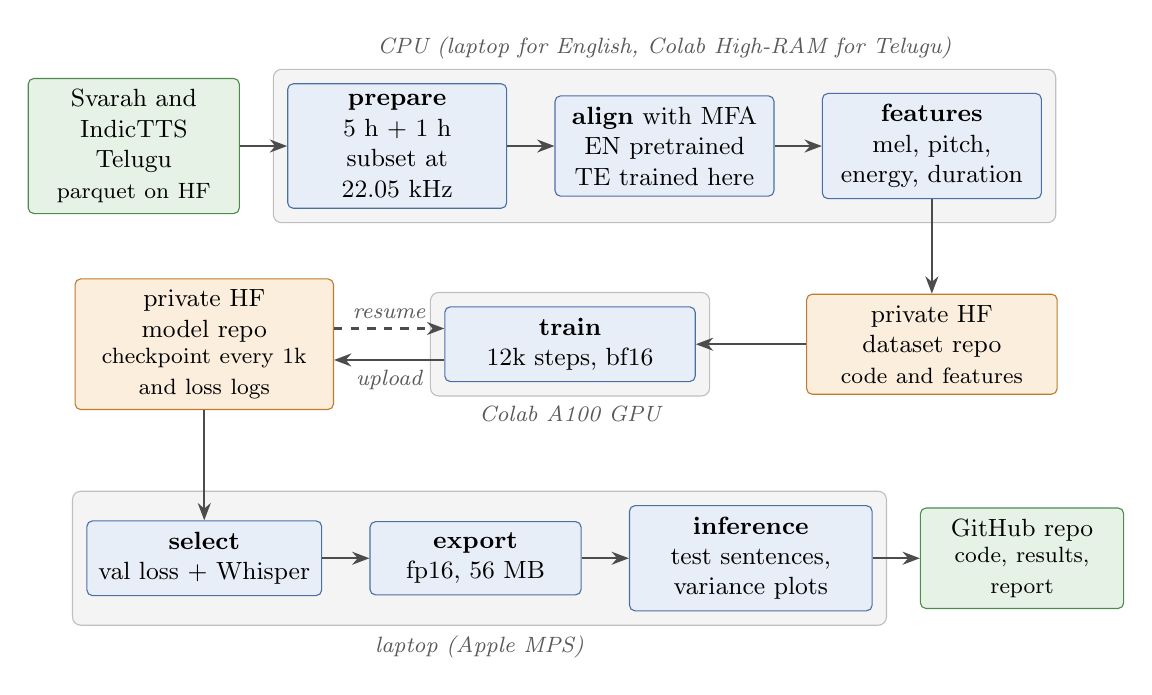
\begin{tikzpicture}[node distance=5mm and 6mm]
  \node[gbox, text width=2.4cm] (src) {Svarah and\\IndicTTS Telugu\\\footnotesize parquet on HF};
  \node[box, text width=2.5cm, right=of src] (prep) {\textbf{prepare}\\5 h + 1 h\\subset at\\22.05 kHz};
  \node[box, text width=2.5cm, right=of prep] (align) {\textbf{align} with MFA\\EN pretrained\\TE trained here};
  \node[box, text width=2.5cm, right=of align] (feat) {\textbf{features}\\mel, pitch,\\energy, duration};
  \begin{scope}[on background layer]
    \node[band, fit=(prep)(align)(feat), label={[note]above:CPU (laptop for English, Colab High-RAM for Telugu)}] (b1) {};
  \end{scope}

  \node[obox, text width=2.9cm, below=12mm of feat] (hfd) {private HF dataset repo\\\footnotesize code and features};
  \node[box, text width=2.9cm, left=14mm of hfd] (train) {\textbf{train}\\12k steps, bf16};
  \node[obox, text width=3.0cm, left=14mm of train] (hfm) {private HF model repo\\\footnotesize checkpoint every 1k\\and loss logs};
  \begin{scope}[on background layer]
    \node[band, fit=(train), label={[note]below:Colab A100 GPU}] (b2) {};
  \end{scope}

  \node[box, text width=2.7cm, below=14mm of hfm] (sel) {\textbf{select}\\val loss + Whisper};
  \node[box, text width=2.4cm, right=of sel] (exp) {\textbf{export}\\fp16, 56 MB};
  \node[box, text width=2.8cm, right=of exp] (inf) {\textbf{inference}\\test sentences,\\variance plots};
  \node[gbox, text width=2.3cm, right=of inf] (gh) {GitHub repo\\\footnotesize code, results,\\report};
  \begin{scope}[on background layer]
    \node[band, fit=(sel)(exp)(inf), label={[note]below:laptop (Apple MPS)}] (b3) {};
  \end{scope}

  \draw[arr] (src) -- (prep);
  \draw[arr] (prep) -- (align);
  \draw[arr] (align) -- (feat);
  \draw[arr] (feat) -- (hfd);
  \draw[arr] (hfd) -- (train);
  \draw[arr] ([yshift=-2mm]train.west) -- node[note, below]{upload} ([yshift=-2mm]hfm.east);
  \draw[arr, dashed] ([yshift=2mm]hfm.east) -- node[note, above]{resume} ([yshift=2mm]train.west);
  \draw[arr] (hfm) -- (sel);
  \draw[arr] (sel) -- (exp);
  \draw[arr] (exp) -- (inf);
  \draw[arr] (inf) -- (gh);
\end{tikzpicture}
\caption{Where each step ran. The dashed arrow resumes training after a disconnect.}
\label{fig:pipeline}
\end{figure}

\subsection{Model}
I started from \href{https://github.com/ming024/FastSpeech2}{ming024/FastSpeech2}, whose code is the first
commit of my repository, unmodified apart from moving its configs to \code{config\_upstream/}. I kept its architecture (Figure~\ref{fig:arch}). The encoder and decoder
(\code{transformer/}), the variance adaptor with its duration, pitch and energy predictors and length regulator
(\code{model/modules.py}), the post-net, the loss, the Noam schedule, the feature extraction and the universal
HiFi-GAN vocoder all come from it, and the speed-ups and bug fixes listed below are my changes to them, besides small edits for newer library versions.

Where ming024 and the FastSpeech~2 paper differ (Table~\ref{tab:paper}), I took the paper's decoder depth and
batch size and kept ming024's phoneme-level pitch and energy, post-net and HiFi-GAN. Phoneme-level values are
also what the assignment asks me to plot. The model has 29.4\,M parameters for English and 29.3\,M for Telugu,
which needs no speaker embedding.

\begin{table}[!htbp]
\centering\small
\begin{tabularx}{\textwidth}{>{\raggedright\arraybackslash}p{4.3cm}XXX}
\toprule
& \textbf{FastSpeech 2 paper} & \textbf{ming024} & \textbf{my setup} \\
\midrule
Encoder and decoder & 4 and 4 FFT blocks & 4 and 6 & 4 and 4 (paper) \\
Hidden size, heads, conv filter and kernel & 256, 2, 1024, 9 & 256, 2, 1024, 9 and 1 & ming024 \\
Encoder and decoder dropout & 0.1 & 0.2 & 0.2 (ming024) \\
Variance predictors & 2 conv layers, kernel 3, 256 filters, dropout 0.5 & same & same \\
Pitch and energy & frame level, wavelet pitch spectrogram, log-scale pitch bins & phoneme level, linear bins & phoneme level (ming024) \\
Post-net & none & 5 conv layers & ming024 \\
Vocoder & Parallel WaveGAN & HiFi-GAN & HiFi-GAN \\
Batch size & 48 & 16 & 48 (paper) \\
Optimiser & Adam (0.9, 0.98, $10^{-9}$), Noam schedule & same, plus annealing & same, plus annealing \\
Training data and length & 24 h, 160k steps & 24 h, 900k steps & 5 h, 12k steps \\
\bottomrule
\end{tabularx}
\caption{Paper, ming024 and my setup.}
\label{tab:paper}
\end{table}

\begin{figure}[!htbp]
\centering
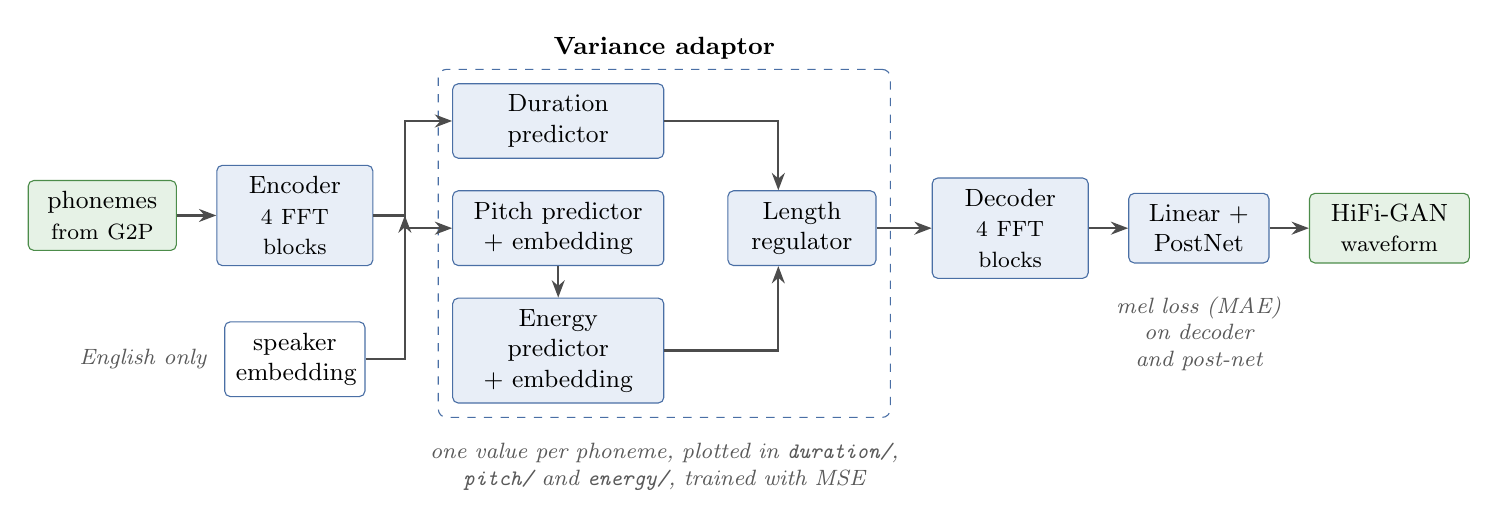
\begin{tikzpicture}[node distance=4mm and 5mm]
  \node[gbox, text width=1.6cm] (ph) {phonemes\\\footnotesize from G2P};
  \node[box, text width=1.7cm, right=of ph] (enc) {Encoder\\\footnotesize 4 FFT blocks};
  \node[box, text width=1.5cm, below=7mm of enc, fill=white] (spk) {speaker\\embedding};
  \node[box, text width=2.4cm, right=10mm of enc, yshift=12mm] (dur) {Duration predictor};
  \node[box, text width=2.4cm, below=of dur] (pit) {Pitch predictor\\+ embedding};
  \node[box, text width=2.4cm, below=of pit] (ene) {Energy predictor\\+ embedding};
  \node[box, text width=1.6cm, right=8mm of pit] (lr) {Length\\regulator};
  \begin{scope}[on background layer]
    \node[draw=blkb, dashed, rounded corners=3pt, fit=(dur)(pit)(ene)(lr), inner sep=5pt, label={[font=\small\bfseries]above:Variance adaptor}] (va) {};
  \end{scope}
  \node[box, text width=1.7cm, right=7mm of lr] (dec) {Decoder\\\footnotesize 4 FFT blocks};
  \node[box, text width=1.5cm, right=of dec] (post) {Linear +\\PostNet};
  \node[gbox, text width=1.75cm, right=of post] (voc) {HiFi-GAN\\\footnotesize waveform};

  \coordinate (split) at ($(enc.east)+(4mm,0)$);
  \draw[arr] (ph) -- (enc);
  \node[note, left=1mm of spk] {English only};
  \draw[arr] (spk.east) -| (split);
  \draw[thick, draw=black!70] (enc.east) -- (split);
  \draw[arr] (split) |- (dur.west);
  \draw[arr] (split) |- (pit.west);
  \draw[arr] (pit) -- (ene);
  \draw[arr] (ene.east) -| ([xshift=-3mm]lr.south);
  \draw[arr] (dur.east) -| ([xshift=-3mm]lr.north);
  \draw[arr] (lr) -- (dec);
  \draw[arr] (dec) -- (post);
  \draw[arr] (post) -- (voc);

  \node[note, below=2mm of va.south, text width=6cm] {one value per phoneme, plotted in \texttt{duration/}, \texttt{pitch/} and \texttt{energy/}, trained with MSE};
  \node[note, below=3mm of post, text width=2.6cm] {mel loss (MAE) on decoder and post-net};
\end{tikzpicture}
\caption{FastSpeech 2 as I use it. The variance adaptor predicts one duration, pitch and energy value per phoneme.}
\label{fig:arch}
\end{figure}

\subsection{Code organisation}
Each language has its own folder with one \code{config.yaml}, \code{preprocess.py}, \code{train.py} and
\code{inference.py}, replacing upstream's three YAML files and per-dataset scripts. The shared model code lives in
\code{fastspeech2/}. Edits to upstream files are marked with \code{\# [MOD]} comments, and the diff against the first
commit gives the complete record.

\subsection{Changes shared by both languages}
\begin{itemize}
\item \textbf{Devices and speed.} I removed the hard-coded \code{.cuda()} calls so the same code trains on the A100
  and runs inference on my MacBook's Apple GPU. I added bf16 mixed precision, replaced the length regulator's
  per-phoneme Python loop with one \code{repeat\_interleave} and padded batches to fixed multiples. Training ran
  at 8.2 iterations per second, so 12k steps took 24 min 17 s for English and 24 min 20 s for Telugu.
\item \textbf{Bug fixes.} Upstream passed the pitch control to the energy predictor, reused the previous
  utterance's statistics after skipping one, and silently dropped the empty intervals that MFA 2 writes for pauses.
  I fixed all three, so the model now learns pause lengths.
\item \textbf{Reproducibility.} A fixed seed, an explicit train and validation list (\code{split.json}), loss
  logs in CSV with IST timestamps and a standalone evaluation script.
\item \textbf{Colab.} Every checkpoint and the logs are mirrored to a private Hugging Face repository, and
  \code{--resume} continues from the newest one.
\item \textbf{Analysis.} A single-utterance synthesis function returns the variance adaptor's outputs, which I
  plot against values measured on the generated audio. I also export fp16 weights (56 MB instead of 350 MB) so the
  models fit in Git.
\end{itemize}

\subsection{English front-end}
\begin{itemize}
\item \textbf{Pseudo-speakers.} Svarah has no speaker IDs, so I use its eight demographic columns as one. They
  form 115 combinations, close to the 117 speakers its authors report.
\item \textbf{Sentence-level G2P.} I run g2p\_en on the whole sentence, so its POS tagger can choose between
  heteronym pronunciations (Figure~\ref{fig:frontend}). Unknown words get its neural prediction.
\item \textbf{One lexicon.} I build the MFA dictionary from the same g2p\_en and CMUdict, so alignment and
  inference share one phone inventory.
\item \textbf{Normalisation.} I expand clock times and AM/PM before upstream's English cleaners and turn the
  hyphens of spelled-out numbers into spaces, so they do not become pauses.
\end{itemize}

\subsection{Telugu front-end}
\begin{itemize}
\item \textbf{Phone set.} I replaced upstream's Mandarin symbols with 46 Telugu phones, 12 vowels and 34
  consonants, written in lower-case ASCII (\ph{tx} for retroflex, \ph{dh} for aspirated) so they never clash with
  ARPAbet.
\item \textbf{Rule-based G2P} (\code{fastspeech2/text/telugu.py}). Telugu script is close to phonemic, so I wrote
  a parser that walks the aksharas (Figure~\ref{fig:frontend}). Consonants carry an inherent \ph{a} unless a vowel
  sign or virama follows, the anusvara becomes the nasal of the next consonant, and the visarga becomes \ph{h}.
\item \textbf{Numbers and times.} I spell them out in Telugu, including ordinals (\te{12వ} becomes
  \te{పన్నెండవ}) and clock times, where the case ending of \te{గంటలకు} moves onto the minutes.
\item \textbf{Alignment.} No pretrained Telugu MFA model exists, so I trained one on the 6-hour subset with my G2P
  as its dictionary (12{,}168 word types). The trained aligner is in the repository.
\end{itemize}

\begin{figure}[!htbp]
\centering
\begin{tikzpicture}[node distance=4mm and 5mm]
  \node[gbox, text width=3.2cm] (e0) {\emph{The researchers will\\conduct an experiment}};
  \node[box, text width=2.5cm, right=of e0] (e1) {normalise\\\footnotesize english\_cleaners,\\times, AM and PM};
  \node[box, text width=2.5cm, right=of e1] (e2) {g2p\_en\\\footnotesize POS tags mark\\\emph{conduct} as a verb};
  \node[gbox, text width=3.6cm, right=of e2] (e3) {\texttt{K AA0 N D AH1 K T}\\\footnotesize stress on the 2nd syllable\\(the noun in E2a gets\\\texttt{K AA1 N D AH0 K T})};
  \draw[arr] (e0) -- (e1); \draw[arr] (e1) -- (e2); \draw[arr] (e2) -- (e3);
  \node[font=\small\bfseries, anchor=south west] at ($(e0.north west)+(0,1mm)$) {English};

  \node[gbox, text width=3.2cm, below=15mm of e0] (t0) {\te{10:45 గంటలకు}};
  \node[box, text width=2.5cm, right=of t0] (t1) {normalise\\\footnotesize numbers, times,\\ordinals};
  \node[box, text width=2.5cm, right=of t1] (t2) {\te{పది గంటల నలభై\\ఐదు నిమిషాలకు}};
  \node[gbox, text width=3.6cm, right=of t2] (t3) {rule-based G2P\\\footnotesize one akshara at a time\\(see table below)};
  \draw[arr] (t0) -- (t1); \draw[arr] (t1) -- (t2); \draw[arr] (t2) -- (t3);
  \node[font=\small\bfseries, anchor=south west] at ($(t0.north west)+(0,1mm)$) {Telugu};
\end{tikzpicture}

\vspace{5mm}
\small
\begin{tabular}{cccc>{\raggedright\arraybackslash}p{7.2cm}}
\toprule
\multicolumn{5}{l}{Akshara by akshara, \te{బలంగా} (“firmly”, T2a) and \te{న్యూరో} (the start of T1)} \\
\midrule
\te{బ} & \te{ల} & \te{ం} & \te{గా} & \\
\ph{b a} & \ph{l a} & \ph{ng} & \ph{g aa} & inherent \ph{a}, the anusvara \te{ం} becomes \ph{ng} before \ph{g}, the vowel sign \te{ా} gives \ph{aa} \\
\midrule
\te{న్} & \te{యూ} & \te{రో} & & \\
\ph{n} & \ph{y uu} & \ph{r oo} & & the virama \te{్} removes the inherent vowel, so \ph{n} joins \ph{y} \\
\bottomrule
\end{tabular}
\normalsize
\caption{Two front-ends. English needs a dictionary, a neural model and POS tags. Telugu needs only rules.}
\label{fig:frontend}
\end{figure}

%=====================================================================
\section{Data}

Table~\ref{tab:data} shows how I selected and split each corpus.
\begin{table}[!htbp]
\centering\small
\begin{tabularx}{\textwidth}{>{\raggedright\arraybackslash}p{2.6cm}XX}
\toprule
& \textbf{English (Svarah)} & \textbf{Telugu (IndicTTS)} \\
\midrule
Source & \code{ai4bharat/Svarah} (gated), 16 kHz & \code{SPRINGLab/IndicTTS\_Telugu}, 48 kHz \\
Speakers & 115 pseudo-speakers (62 F, 53 M, 19 first languages) & one male speaker \\
Filters & 1.5 to 11 s, at least 3 words, plain ASCII, no digit runs over 4 & 1 to 11 s, no Latin letters or digits \\
Candidates & 4{,}341 utterances, 6.27 h & 3{,}262 utterances, 6.21 h \\
Split & stratified by speaker, random utterances to validation until 15.9\% of each speaker's audio & random, first 1 h to validation \\
Train & 3{,}451 utts, 5.00 h & 2{,}625 utts, 5.00 h (one of 2{,}626 failed alignment) \\
Validation & 774 utts, 1.11 h & 531 utts, 1.00 h \\
Overlap & none & none \\
\bottomrule
\end{tabularx}
\caption{Data selection, seeded and committed in \code{<Lang>/raw\_data/split.json}.}
\label{tab:data}
\end{table}

\begin{itemize}
\item \textbf{Length.} The 11 s cap keeps every utterance under the model's 1000-frame limit.
\item \textbf{English filters.} The lower bounds drop one-word voice commands, and long digit strings are read
  digit by digit, which my normaliser does not reproduce.
\item \textbf{English split.} Stratifying by speaker gives every validation speaker a trained embedding, at the cost
  of a validation set of 1.11 h. The median speaker has 1.9 min of training audio and \code{spk073} has the most
  (14.0 min), so \code{spk073} is my inference voice.
\item \textbf{Telugu speaker.} I chose the male speaker for his 48 kHz studio recordings (the female ones are
  16 kHz). His F0 averages 190 Hz, high for a man, so I listened to random clips and confirmed the label.
\item \textbf{Dataset card.} The card lists 4.47 h of male speech, but the WAV headers add up to 12.8 h, plenty
  for a 6-hour subset.
\end{itemize}

\subsection{Preprocessing}
Each \code{preprocess.py} runs three stages.
\begin{enumerate}
\item \textbf{prepare} resamples the audio to 22.05 kHz, peak-normalises it and writes the normalised transcript
  for MFA.
\item \textbf{align} runs MFA 3.4 with a wide beam (100, retry 400), with the pretrained \code{english\_us\_arpa}
  model and my g2p\_en lexicon (6{,}699 word types) for English and my own model for Telugu, whose training took 2.8 h on an 8-core
  Colab CPU.
\item \textbf{features} trims silence at the alignment boundaries and computes 80-band log-mels (FFT 1024, hop
  256), WORLD pitch and STFT energy, both averaged per phoneme and z-normalised. After trimming, training and
  validation together hold 5.67 h of English and 5.00 h of Telugu speech.
\end{enumerate}
Three corpus facts matter later (\code{scripts/corpus\_stats.py}). English pitch spreads widely (mean 178.5 Hz,
standard deviation 56.8) because men and women are pooled. Svarah's pauses are long-tailed (median 151 ms,
90th percentile 650 ms), the mark of hesitant reading, while the Telugu speaker's are short and even (186 and
360 ms). And some Telugu phones are rare, such as \ph{au} with 160 of 203{,}424 tokens.

\subsection{Training configuration}
\begin{table}[!htbp]
\centering\small
\begin{tabular}{ll}
\toprule
Model & 4 encoder and 4 decoder FFT blocks, 29.4\,M parameters (29.3\,M for Telugu) \\
Optimiser & Adam (0.9, 0.98, $10^{-9}$), Noam schedule, 4000 warm-up steps, $\times$0.3 at 6k, 8k and 10k \\
Batch & 48 utterances, gradient clipping at 1.0 \\
Steps & 12{,}000, validation every 500, checkpoint every 1000 \\
Losses & MAE on mel and post-net mel, MSE on phoneme-level pitch, energy and log-duration \\
Precision & bf16 autocast, fp32 weights \\
Hardware & Colab A100 (40 GB), 24 min per language on 1 Nov 2026 (20:09 to 20:34 IST) \\
\bottomrule
\end{tabular}
\caption{Training setup, identical for both languages.}
\end{table}

The paper trains for 160k steps and ming024 for 900k, both on 24 hours of LJSpeech. With a fifth of that data I
expected convergence within a few thousand steps, so I gave each language 12k, enough to find the validation
minimum and see what follows. I lower the learning rate at 6k, 8k and 10k so the weights settle near the end.

%=====================================================================
\section{Loss curves}
\label{sec:loss}

\begin{figure}[!htbp]
\centering
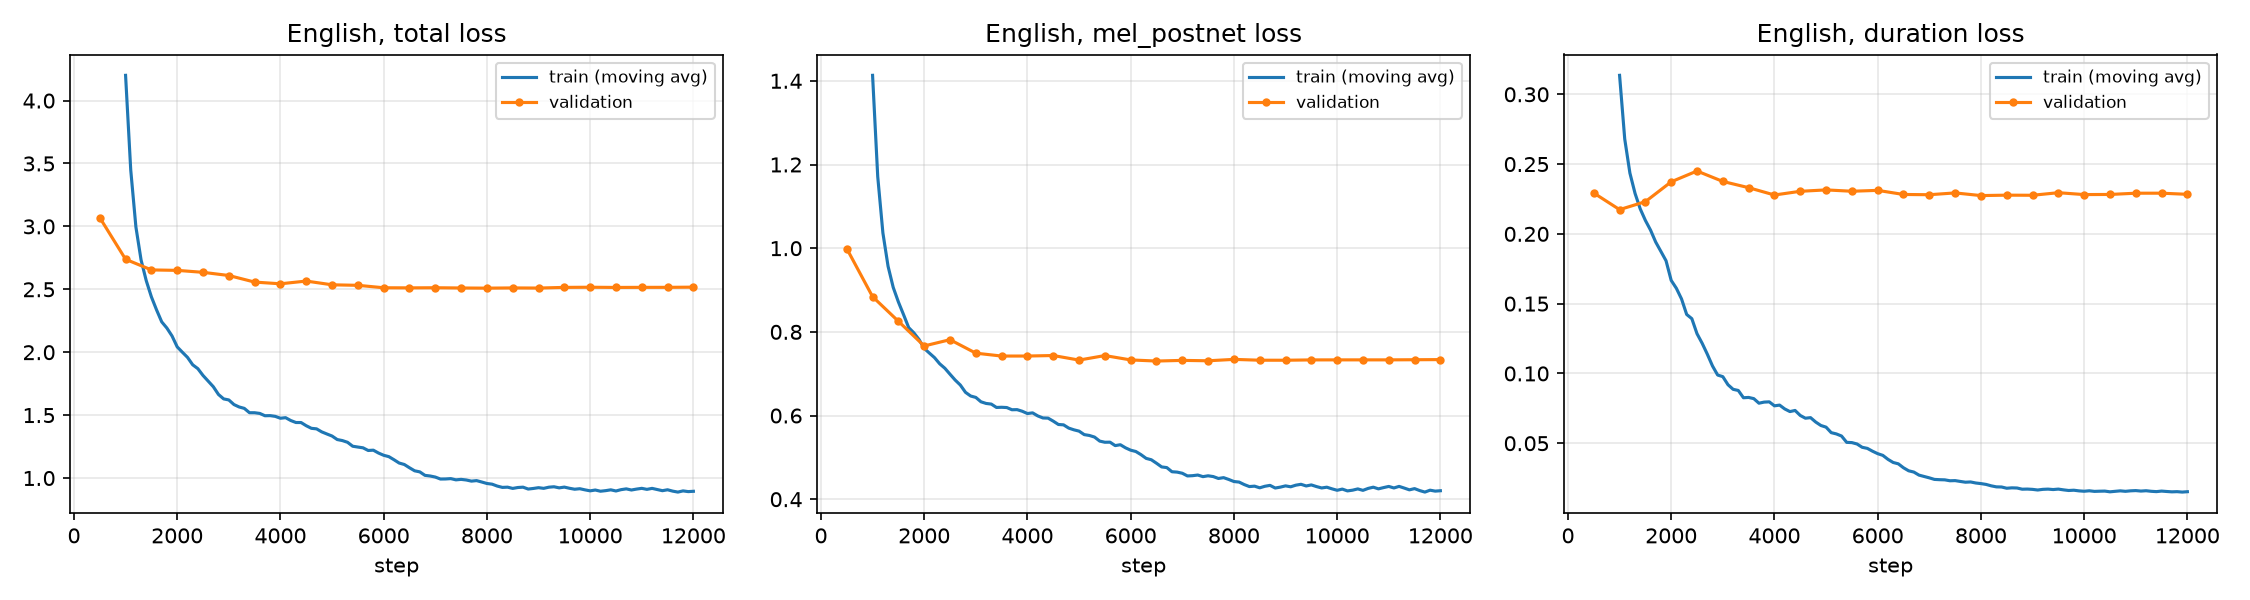
\includegraphics[width=\textwidth]{English/train_vs_val_loss.png}\\[2pt]
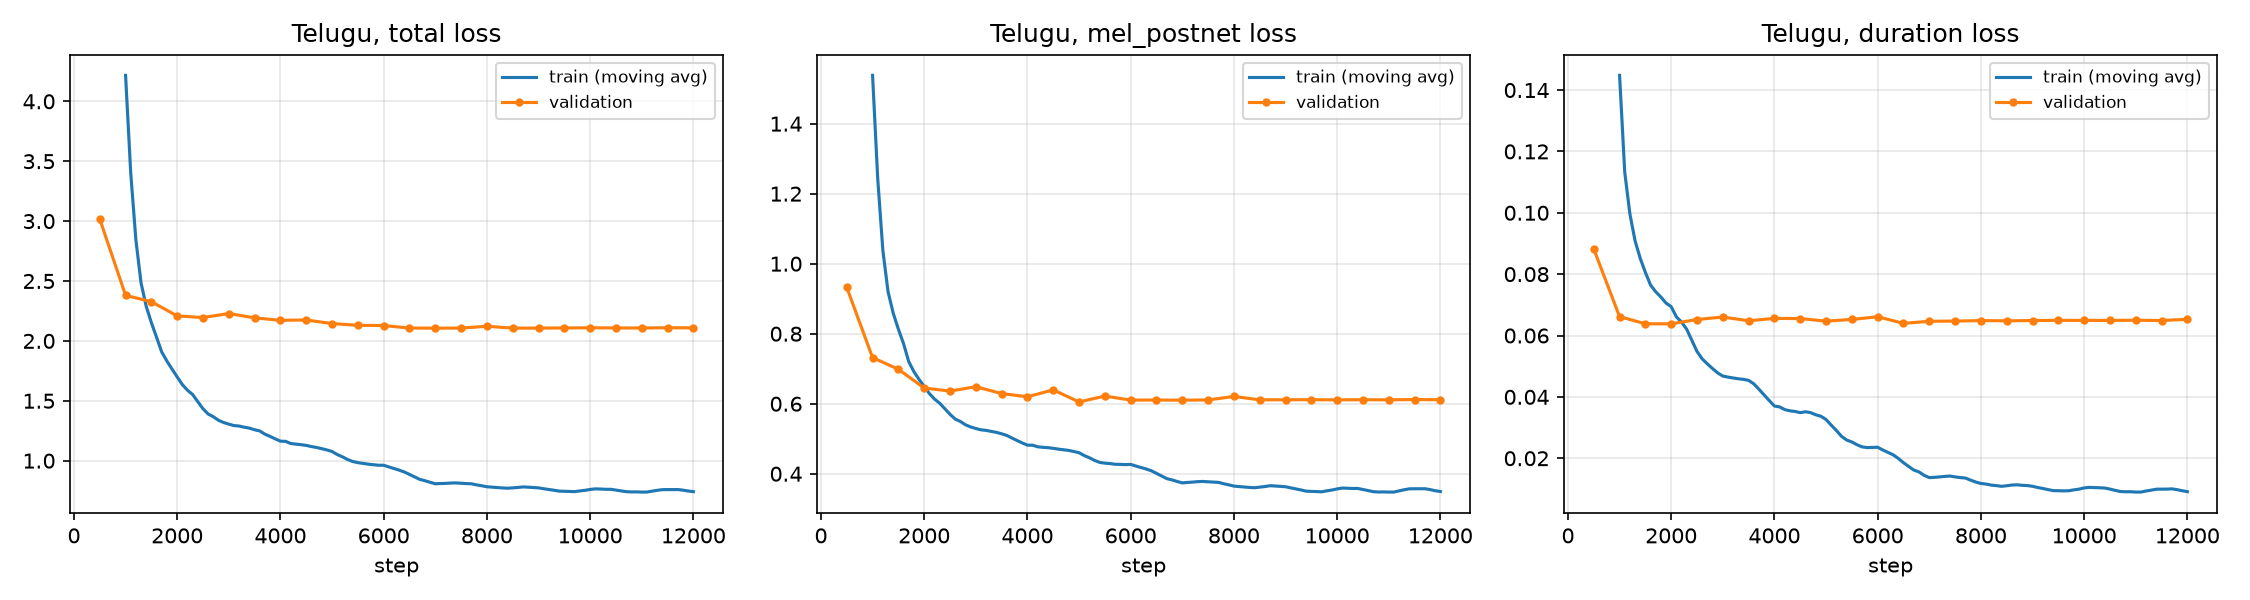
\includegraphics[width=\textwidth]{Telugu/train_vs_val_loss.png}
\caption{Training (smoothed) and validation loss. English top, Telugu bottom.}
\label{fig:loss}
\end{figure}


\paragraph{Convergence.} Validation loss falls through the 4000-step warm-up and levels off by 6.5k
(Figure~\ref{fig:loss}, Table~\ref{tab:loss}). Among the saved checkpoints it is lowest at 8k for English (2.509)
and 7k for Telugu (2.106), after 113 and 130 passes over the data. Telugu touches the same 2.106 again at 8.5k, and
both stay within 1\% of their minimum to the end. Two stretches are unsteady. While the learning rate peaks,
Telugu validation rises at 3k and English at 4.5k, and the English checkpoint from 3k is barely intelligible
(Table~\ref{tab:asr}). Telugu also jumps once at 8k (2.106 to 2.122) and is back by 8.5k. Training never
diverged.

\begin{table}[!htbp]
\centering\small
\begin{tabular}{llrrrrrr}
\toprule
& step & total & mel & post-net & pitch & energy & duration \\
\midrule
English train & 9k & 0.929 & 0.436 & 0.436 & 0.019 & 0.023 & 0.016 \\
English val   & 8k & \textbf{2.509} & 0.734 & 0.734 & 0.439 & 0.374 & 0.227 \\
English val   & 9k & 2.510 & 0.732 & 0.732 & 0.440 & 0.378 & 0.228 \\
English val   & 12k & 2.517 & 0.734 & 0.734 & 0.442 & 0.380 & 0.228 \\
\midrule
Telugu train  & 6k & 0.948 & 0.426 & 0.426 & 0.040 & 0.034 & 0.022 \\
Telugu val    & 7k & \textbf{2.106} & 0.610 & 0.610 & 0.598 & 0.223 & 0.065 \\
Telugu val    & 6k & 2.128 & 0.611 & 0.610 & 0.615 & 0.226 & 0.066 \\
Telugu val    & 12k & 2.109 & 0.612 & 0.611 & 0.598 & 0.222 & 0.065 \\
\bottomrule
\end{tabular}
\caption{Losses at key steps. Bold is the lowest validation total at a saved checkpoint.}
\label{tab:loss}
\end{table}

\paragraph{Overfitting.} Training loss keeps falling after validation stops (English 1.07 at 6k to 0.93 at 9k,
Telugu 0.95 to 0.72). The variance predictors overfit hardest. Training pitch loss reaches 0.019 for English and
0.016 for Telugu while validation stays at 0.44 and 0.60. The pitch targets are z-normalised to unit variance, so 0.60
means the predictor accounts for only about 40\% of the phoneme-level pitch variance in unseen sentences. It learns
what generalises early and then memorises the training sentences, which is why I chose among the plateau
checkpoints by intelligibility instead of taking the last one.

\paragraph{The two languages.} Telugu has the lower mel loss (0.61 against 0.73) and duration loss (0.065 against
0.23), because one studio speaker is far easier to model than 115 amateurs with two minutes each. English has the
lower pitch loss (0.44 against 0.60) largely because its speaker embedding absorbs the male and female difference.
Telugu pitch is pure intonation, which is harder to predict from text.

\paragraph{Picking the checkpoints.} Validation loss feeds in the true durations, pitch and energy, so it does not
show how the synthesis sounds. The last cell of each training notebook therefore synthesises 60 validation
sentences from every checkpoint and transcribes them with Whisper (Table~\ref{tab:models}). Among the
checkpoints after the plateau begins at 6k, I took the lowest word error rate, English 9k and Telugu 6k
(Table~\ref{tab:asr}), and confirmed both by listening.

\begin{table}[!htbp]
\centering\small
\begin{tabular}{lrrr|rrr}
\toprule
& \multicolumn{3}{c|}{\textbf{English} (674 words)} & \multicolumn{3}{c}{\textbf{Telugu} (1906 words)} \\
step & val loss & WER & CER & val loss & WER & CER \\
\midrule
3k & 2.610 & 84.9 & 39.8 & 2.228 & 24.6 & 15.2 \\
6k & 2.512 & 15.1 & 8.1 & 2.128 & \textbf{23.9} & 15.0 \\
7k & 2.512 & 15.6 & 8.9 & \textbf{2.106} & 25.8 & 16.1 \\
8k & \textbf{2.509} & 17.4 & 9.6 & 2.122 & 25.1 & 15.0 \\
9k & 2.510 & \textbf{15.0} & 7.7 & 2.107 & 26.0 & 16.5 \\
10k & 2.516 & 15.1 & 8.6 & 2.110 & 26.9 & 17.4 \\
12k & 2.517 & 16.0 & 8.6 & 2.109 & 28.1 & 17.7 \\
\midrule
\multicolumn{7}{l}{\emph{against the original transcripts (680 English words), on my MacBook}} \\
selected & & 15.1 & 8.6 & & 24.4 & 14.9 \\
real speech & & 7.1 & 4.1 & & 25.4 & 16.7 \\
\bottomrule
\end{tabular}
\caption{Picking the checkpoint. Whisper error rates (\%) on 60 held-out sentences.}
\label{tab:asr}
\end{table}

The checkpoint rows come from Colab and score the synthesis against the normalised transcripts. On my MacBook I
also scored the selected checkpoints and the real recordings against the original transcripts. Synthetic English
makes twice as many errors as real English, while synthetic Telugu scores slightly better than real Telugu,
because the speaker strays from his transcripts and Whisper's Telugu is weak. The Telugu numbers therefore only
rank checkpoints against each other.

%=====================================================================
\section{Test sentences}
\label{sec:va}

I synthesised all ten sentences with the selected checkpoints and no prosody control, using \code{spk073} for
English. The audio and plots are in \code{Results/<Lang>/}. Each sentence has three plots, the predicted duration
of every phoneme (pauses in grey) on top, and below it the predicted pitch and energy per phoneme (red steps) over
the values measured on the generated audio (grey). The two agree closely on voiced phones, so the decoder and vocoder do
what the variance adaptor asks.

Three patterns hold across all ten sentences. Vowels are predicted 1.6 to 2.4 times as loud as consonants, with
stop closures and voiceless fricatives at the bottom. Pitch falls through most sentences (E1 and E3 end on a rise) and
energy falls with it, ending at 17 to 67\% of its opening level in eight sentences. And the last syllable before a pause or the end is
stretched. Below, “ASR” is Whisper's transcript and “Listening” is what I heard.

\subsection{English}
\begin{table}[!htbp]
\centering\small
\begin{tabular}{lrrrl}
\toprule
ID & duration & phones & F0 (Hz) & pauses \\
\midrule
E1 & 5.18 s & 87 & 130 $\pm$ 15 & none \\
E2a & 3.40 s & 51 & 128 $\pm$ 12 & none \\
E2b & 3.59 s & 56 & 136 $\pm$ 17 & none \\
E3 & 2.64 s & 37 & 136 $\pm$ 18 & none \\
E4 & 6.61 s & 81 & 132 $\pm$ 24 & 755 ms at the comma \\
\bottomrule
\end{tabular}
\caption{English test sentences (spk073, checkpoint 9k).}
\end{table}

\paragraph{E1, long and rare words} (Figure~\ref{fig:va-E1}).
\begin{itemize}
\item \textbf{Duration.} CMUdict gives \emph{antidisestablishmentarianism} 28 phones, spoken in 1.67 s at an average
  of 60 ms each with no break. The vowel of the final \emph{-ble} in \emph{considerable} shrinks to 12 ms, leaving
  a syllabic \emph{l} as in natural speech. \emph{Proceedings} ends unevenly, with its \ph{S} at 151 ms and its final \ph{NG Z} at 116 and
  162 ms.
\item \textbf{Pitch and energy.} Pitch starts at 152 Hz, peaks inside the long word and falls to 107 Hz, then rises
  again to 156 Hz near the end. Energy barely fades (108 to 100), so the sentence never settles.
\item \textbf{ASR.} “The entire disestablishmentism movement in considerable momentum during the parliamentary
  proceedings.”
\item \textbf{Listening.} The long word is mushy and takes effort. \emph{Proceedings} sounds odd with a stretched
  “cee”, matching the long \ph{S} and the unsettled ending. A mild buzz runs throughout.
\end{itemize}
\vaplots{English}{E1}{A 28-phone word in one even rush}

\needlines{4}\paragraph{E2a and E2b, the heteronym \emph{conduct}} (Figures~\ref{fig:va-E2a} and \ref{fig:va-E2b}).
\begin{itemize}
\item \textbf{Front-end.} g2p\_en tags the noun as \ph{K AA1 N D AH0 K T} and the verb as \ph{K AA0 N D AH1 K T}.
\item \textbf{Duration.} Length does not mark stress. The verb's stressed \ph{AH1} lasts 35 ms against 81 ms for
  the noun's \ph{AH0}. \emph{Orchestra's} is unhurried (604 ms), and the final \ph{S} of \emph{audience} is held
  for 209 ms.
\item \textbf{Pitch and energy.} Pitch is nearly flat across both forms, and energy does not separate them either.
  The second vowel is louder in both, 101 against 83 in the verb and 108 against 85 in the noun. The contrast comes
  from the stress-marked phones themselves, since \ph{AA1} and \ph{AA0} are different symbols to the model. E2b
  peaks in pitch on \emph{researchers} (181 Hz).
\item \textbf{ASR.} Both sentences come back word for word.
\item \textbf{Listening.} Both are clear and natural with a faint buzz, and \emph{orchestra} sounds relaxed. E2b is
  clearly con-DUCT, while E2a is only weakly CON-duct, which fits its long unstressed second vowel (81 ms).
\end{itemize}
\vaplots{English}{E2a}{\emph{Conduct} as a noun, with weak stress}
\vaplots{English}{E2b}{\emph{Conduct} as a verb, stressed on the second syllable}

\needlines{4}\paragraph{E3, the split word “rhyth m”} (Figure~\ref{fig:va-E3}).
\begin{itemize}
\item \textbf{Front-end.} I kept the text as given, two spaces included. g2p\_en guesses \ph{R AY1 DH} for “rhyth” and reads the lone
  “m” as the letter \ph{EH1 M}, so the model is asked to say “rythe em”.
\item \textbf{Duration.} The two pieces run together with no pause, and the last vowel of \emph{unexpectedly} is
  stretched to 151 ms.
\item \textbf{Pitch and energy.} The spurious “em” takes the pitch peak (171 Hz), which makes it stand out. Pitch
  drops to 110 Hz and climbs back to 150 Hz on the final \emph{-ly}, so the sentence ends on a rise. Energy halves
  towards the end.
\item \textbf{ASR.} “The item of the orchestra changed unexpectedly.”
\item \textbf{Listening.} “Ryth-em” instead of \emph{rhythm}, otherwise clear. The acoustic model says exactly what
  the front-end gives it, so the fix is a spelling-correction step before G2P.
\end{itemize}
\vaplots{English}{E3}{“Rhyth m” read as “ryth-em”}

\needlines{4}\paragraph{E4, numbers, time, date and a code-mixed word} (Figure~\ref{fig:va-E4}).
\begin{itemize}
\item \textbf{Front-end.} “10:45~AM” becomes “ten forty five ay em” and the date “twelve November twenty twenty
  six”. “Andaroo” (\te{అందరూ}, “everyone”) is anglicised as \ph{AE0 N D AA1 R OW0}.
\item \textbf{Duration.} The comma after 2026 becomes a 755 ms pause, the worst prosodic error in the test set.
  The duration predictor inherited it from Svarah's long-tailed pauses, while the Telugu model gives its comma
  406 ms. “Andaroo” is squeezed into 302 ms.
\item \textbf{Pitch and energy.} The widest English range (104 to 212 Hz), peaking on \emph{meeting}, with only a
  small reset after the pause (124 to 143 Hz), so the second clause sounds like an afterthought. “AM” is predicted
  quiet (91 and 79 against a vowel average of 102).
\item \textbf{ASR.} “The meeting will start at 10 45 when amount while member for the 26th someone else should
  arrive one time.”
\item \textbf{Listening.} “AM” is too hushed to tell from PM, and “andaroo” is rushed and hard to follow. English
  also has no dental \ph{d}, so the word can never sound like \te{అందరూ}. The quiet “AM” comes from the energy
  predictor, while “andaroo” needs a fix in the front-end.
\end{itemize}
\vaplots{English}{E4}{The 755 ms pause after 2026}

\needlines{8}
\subsection{Telugu}
\begin{table}[!htbp]
\centering\small
\begin{tabular}{lrrrl}
\toprule
ID & duration & phones & F0 (Hz) & pauses \\
\midrule
T1 & 4.52 s & 66 & 197 $\pm$ 39 & none \\
T2a & 2.10 s & 31 & 190 $\pm$ 33 & none \\
T2b & 2.46 s & 37 & 183 $\pm$ 41 & none \\
T3 & 1.88 s & 31 & 195 $\pm$ 37 & none \\
T4 & 7.98 s & 128 & 185 $\pm$ 27 & 406 ms at the comma \\
\bottomrule
\end{tabular}
\caption{Telugu test sentences (checkpoint 6k).}
\end{table}

\paragraph{T1, a long technical loanword} (Figure~\ref{fig:va-T1}).
\begin{itemize}
\item \textbf{Front-end.} The G2P reads \te{న్యూరోఫార్మకోలాజికల్} as spelled, with an aspirated \ph{ph} where many
  speakers say [f].
\item \textbf{Duration.} The loanword takes 1.43 s and keeps its long vowels long (70 to 116 ms) and short ones
  short (35 to 46 ms). The \ph{au} of \te{ఔషధాల} is the longest vowel in the sentence (174 ms).
\item \textbf{Pitch and energy.} The largest fall of all ten sentences, from 278 Hz on \te{న్యూరో} to 110 Hz,
  with small resets at the start of later words, a pattern the model learned from the speaker. Energy follows,
  but the \ph{au} is predicted at only 56\% of the average vowel, so it comes out weak.
\item \textbf{ASR.} Whisper writes “Neuro Pharmacological” and renders \te{ఔషధాల} as \te{ఉషదాల}.
\item \textbf{Listening.} The loanword is clear, with “pha” rather than “fa”. \te{ఔషధాల} comes out as
  “ushadhaala”, the \ph{au} turned into “uu”. With 160 training examples the model never learned this diphthong.
\end{itemize}
\vaplots{Telugu}{T1}{The loanword peaks first, and \te{ఔ} comes out weak}

\needlines{4}\paragraph{T2a and T2b, \te{పట్టు} as “grip” and “silk”} (Figures~\ref{fig:va-T2a} and \ref{fig:va-T2b}).
\begin{itemize}
\item \textbf{Front-end.} Both meanings sound the same, so both sentences correctly get \ph{p a tx tx u}.
\item \textbf{Duration.} \te{పట్టు} lasts 279 and 302 ms, with a long closure for the doubled \ph{tx}.
\item \textbf{Pitch and energy.} \te{పట్టు} sits high in both (228 and 254 Hz), and both sentences fall to
  118 Hz. T2a stresses the intensifier \te{చాలా} (energy 134), and the doubled \ph{tx} shows as a silent gap in
  both.
\item \textbf{ASR.} Both correct apart from word spacing, and in T2a Whisper writes \te{పై అతని} as \te{పైయతని}.
\item \textbf{Listening.} Both natural, with \te{పట్టు} identical in the two and only brief traces of buzz.
\end{itemize}
\vaplots{Telugu}{T2a}{\te{పట్టు} as grip, with the stress on \te{చాలా}}
\vaplots{Telugu}{T2b}{\te{పట్టు} as silk, pronounced the same}

\needlines{4}\paragraph{T3, the split word \te{అడ విలో}} (Figure~\ref{fig:va-T3}).
\begin{itemize}
\item \textbf{Front-end.} The two halves convert to \ph{a dx a v i l oo}, exactly the phones of \te{అడవిలో}, and
  no pause is inserted at the space. Telugu script maps to sound syllable by syllable, so the split that broke
  E3 is harmless here.
\item \textbf{Duration.} 16.5 phones per second, with the doubled \ph{sh sh} of \te{నిశ్శబ్దంగా} held for 209 ms.
\item \textbf{Pitch and energy.} The subject \te{పులి} has the highest pitch of all ten sentences (288 Hz). Pitch
  runs smoothly across the space, and the word starts with the loudest syllable of the sentence.
\item \textbf{ASR.} Whisper writes \te{అడవిలో} as one word.
\item \textbf{Listening.} One natural word, no break.
\end{itemize}
\vaplots{Telugu}{T3}{\te{అడ విలో} joined into one word}

\needlines{4}\paragraph{T4, numbers, date and time} (Figure~\ref{fig:va-T4}).
\begin{itemize}
\item \textbf{Front-end.} “2026” becomes \te{రెండు వేల ఇరవై ఆరు}, “\te{12వ}” becomes \te{పన్నెండవ} and
  “\te{10:45 గంటలకు}” becomes \te{పది గంటల నలభై ఐదు నిమిషాలకు}.
\item \textbf{Duration.} The longest sentence (7.98 s). Vowels inside the numbers shrink to 23 ms, the pace of a
  familiar date, and the comma gets a natural 406 ms.
\item \textbf{Pitch and energy.} Pitch falls to 124 Hz before the comma and resets fully to 213 Hz on
  \te{సమయానికి}, so the second clause starts afresh. Energy follows the same two-phrase shape.
\item \textbf{ASR.} Every number comes back recognisably in words, with small spelling slips such as \te{రిండు}
  for \te{రెండు}.
\item \textbf{Listening.} Clear, numbers correct, with one brief buzz at the comma.
\end{itemize}
\vaplots{Telugu}{T4}{A full pitch reset after the comma}

\subsection{A second opinion from audio models}
\label{sec:second}
To check my ears, I ran the ten clips through Whisper and two Gemini models, none of them fine-tuned
(Table~\ref{tab:models}). Whisper transcribed them. Gemini Argon High, in the Gemini app, first transcribed them
blind and then answered questions on intelligibility, naturalness, buzz and one point per sentence. Gemini 3
Flash, through the API, got the same questions. The prompts are in Appendix~\ref{app:prompts} and the unedited
replies in \code{Report/listening\_checks/}.

\begin{table}[!htbp]
\centering\footnotesize
\begin{tabularx}{\textwidth}{>{\raggedright\arraybackslash}p{2.6cm}>{\raggedright\arraybackslash}p{4.7cm}X}
\toprule
\textbf{Model} & \textbf{Exact version} & \textbf{Settings} \\
\midrule
Whisper small.en & \code{openai/whisper-small.en}, revision \code{e872752}, 241.7\,M parameters & English only, greedy decoding, fp32 \\
Whisper large-v3-turbo & \code{openai/whisper-large-v3-turbo}, revision \code{41f01f3}, 808.9\,M parameters & language forced to Telugu, greedy decoding, fp32 \\
Gemini 3 Flash & \code{gemini-3-flash-preview}, Gemini API, \code{google-genai} 2.34.0 & one request, temperature 0, 2 Nov 2026 \\
Gemini Argon High & Argon High in the Gemini app (Google AI Pro) & default settings, two messages \\
\bottomrule
\end{tabularx}
\caption{The audio models, all used as released. For the test clips, Whisper ran on my MacBook in \code{transformers} 5.22.1 with PyTorch 2.15.0.}
\label{tab:models}
\end{table}

\begin{table}[!htbp]
\centering\footnotesize
\begin{tabularx}{\textwidth}{l>{\raggedright\arraybackslash}X>{\raggedright\arraybackslash}X>{\raggedright\arraybackslash}X>{\raggedright\arraybackslash}X}
\toprule
& \textbf{My listening} & \textbf{Whisper} & \textbf{Gemini Argon High} & \textbf{Gemini 3 Flash} \\
\midrule
E1 & long word mushy, \emph{proceedings} odd, mild buzz & recovers most of the long word & long word only partly intelligible, strong buzz & long word clear, end of \emph{proceedings} stretched, mild buzz \\
E2a & clear, CON-duct but weakly & word for word & CON-duct, strong buzz & CON-duct, \emph{orchestra} natural, no buzz \\
E2b & clear, con-DUCT & word for word & con-DUCT, strong buzz & con-DUCT, no buzz \\
E3 & “ryth-em” & “item” & “ride-em” & “rhyth-um” with a break \\
E4 & AM hushed, \emph{andaroo} rushed, long gap & AM and \emph{andaroo} lost & AM unclear, \emph{andaroo} unintelligible, gap of a full second & AM clear, \emph{andaroo} with a hard English d, pause too long \\
T1 & \te{ఔ} sounds like “uu” & writes \te{ఉషదాల} & clean “au” & clean “au” \\
T2a & natural, slightly robotic & correct apart from spacing and \te{పైయతని} & natural, \te{పయతని} joined, no buzz & natural, no buzz \\
T2b & natural & correct apart from spacing & natural, no buzz & natural, no buzz \\
T3 & one word, natural & \te{అడవిలో} as one word & one word & break inside the word \\
T4 & clear, numbers right, tiny buzz & numbers recognisable & numbers right, glitch at the comma & numbers right \\
\bottomrule
\end{tabularx}
\caption{My ears against three audio models.}
\label{tab:second}
\end{table}

The models mostly heard what I heard (Table~\ref{tab:second}). Both Gemini models agree on the stress of \emph{conduct}, the over-long
pause in E4 and the English “d” in “andaroo”, and Gemini 3 Flash also hears the stretched end of
\emph{proceedings}. Whisper and Argon High, like me, could not make out “AM” or “andaroo”. Everyone finds T2b
and the numbers in T4 right and T2a natural, although Whisper and Argon High both join \te{పై} and \te{అతని}.
Both Gemini models find less buzz in Telugu than in English.

Two disagreements remain, and I am confident the models are wrong in both. In T1 both Gemini models report a clean
“au” in \te{ఔషధాల}. I clearly hear “uu”, and Whisper wrote \te{ఉషదాల}, which matches what I hear. Gemini writes the word it knows, the same
habit that made Argon High replace sentence endings with plausible guesses. And Gemini 3 Flash hears a break
inside the split words of E3 and T3, where the audio has no pause and the pitch runs smoothly across. It was
apparently reacting to the space in the prompt text.

Argon High also replaced the last word or two of most clips with guesses (“debates” for “proceedings”) and
called several Telugu clips cut off, endings that Whisper and Gemini 3 Flash heard in full. I left its comments on
endings out.

%=====================================================================
\section{English and Telugu compared}
\begin{itemize}
\item \textbf{Data.} One studio speaker is a far easier target than 115 amateurs with two minutes each. Telugu has
  the lower mel loss (0.61 against 0.73), a third of the duration loss (0.065 against 0.23) and shorter pauses
  (406 against 755 ms at the comma).
\item \textbf{Text processing} (Figure~\ref{fig:frontend}). Telugu spelling is nearly phonemic, so about 200 lines
  of rules give a complete G2P that shrugs off split and unseen words (T3). English needs a dictionary, a neural
  model and POS tagging, and it breaks on corrupted input (E3) and foreign words (E4). The Telugu G2P's blind
  spots are loanwords (\ph{ph} for [f]) and cross-word sandhi.
\item \textbf{Alignment.} English uses an aligner trained on thousands of hours. The Telugu aligner learned from the
  same 6 hours it aligned, yet handled 3{,}156 of 3{,}157 utterances with sharp phoneme boundaries.
\item \textbf{Prosody.} Telugu has the wider pitch range (standard deviation 15 to 23\% of the mean against 10 to
  19\% for English), stronger word-initial prominence and a full reset after a comma (T4). English stress comes
  from the stress-marked phones, not from the predicted prosody (E2), and English resets weakly after its pause
  (E4).
\item \textbf{Quality.} Telugu sounds natural with rare traces of buzz, English clear with a mild buzz throughout.
  The buzz most likely comes from the universal HiFi-GAN, which never heard either voice. English suffers more,
  which fits its less accurate mels (validation mel loss 0.73 against 0.61) across many speakers and recording
  conditions.
\item \textbf{Intelligibility.} Scored against the original transcripts of the same 60 sentences, Whisper makes
  2.1 times as many errors on synthetic English as on real English (15.1\% against 7.1\% WER).
\end{itemize}

%=====================================================================
\section{Limitations and improvements}
\begin{itemize}
\item \textbf{Overfitting after 6k steps}, mostly in the variance predictors. The likely remedies are more dropout there,
  pitch and energy augmentation, or pretraining on a larger corpus and fine-tuning on the 5-hour subsets.
\item \textbf{Variance predictor slips in E4}, the 755 ms pause inherited from Svarah's hesitant reading and the
  quiet “AM”. Capping long pause targets should fix the pause.
\item \textbf{Text processing} causes the split word in E3 and the rushed “andaroo” in E4, and reads the
  loanword in T1 with \ph{ph}. A word-joining pass, transliteration of code-mixed words and an exception list for
  loanwords would deal with them.
\item \textbf{Rare Telugu phones} such as \ph{au} (160 tokens), which T1 shows the model has not learned.
  Selecting the subset for phone coverage should help.
\item \textbf{Uneven English speakers.} Inference uses the best-covered speaker, and those with under a minute of
  data are modelled poorly.
\item \textbf{Abrupt endings.} I trimmed silence from the training audio, so every clip ends within milliseconds
  of its last sound, which some tools clip. Appending a short silence after synthesis avoids this. I left the clips
  exactly as the model produced them.
\item \textbf{Vocoder.} Vocoding ground-truth mels would confirm where the buzz comes from, and fine-tuning
  HiFi-GAN on mels from my models should remove most of it.
\item \textbf{Evaluation.} My listening notes are from one listener. A MOS test with several native speakers is
  the right next step.
\end{itemize}

%=====================================================================
\section{Reproducibility}
\label{sec:repro}
\begin{itemize}
\item \textbf{Environment.} Python 3.11 with MFA 3.4.3 and the packages in \code{requirements.txt} on my MacBook,
  Python 3.13 with PyTorch 2.11 on Colab. All inference and analysis ran on the MacBook's Apple GPU. The
  Whisper checks also need \code{transformers}.
\item \textbf{Configuration.} Every setting for a language is in its \code{config.yaml}.
\item \textbf{Determinism.} Seed 1234 throughout. The train and validation lists, lexicons, the Telugu aligner and
  the feature statistics are committed, and rerunning Telugu data selection on Colab reproduced my split file for
  file.
\item \textbf{Training record.} \code{colab/train\_English.ipynb} and \code{colab/train\_Telugu.ipynb} trained the
  submitted models and keep every output and cell time as Colab printed them. The English notebook shows one failed cell, an NLTK
  tagger missing on a fresh install, which \code{synthesize.py} now downloads by itself. The loss CSVs in \code{<Lang>/logs/} timestamp every logged step.
\item \textbf{Checkpoints.} \code{English/checkpoints/9000\_inference.pth.tar} and\\
  \code{Telugu/checkpoints/6000\_inference.pth.tar} hold the fp16 weights (56 MB each), exported with
  \code{scripts/export\_inference\_ckpt.py}. The full checkpoints and TensorBoard logs are on Hugging Face, and the
  committed results come from exactly these files.
\item \textbf{Commands.}
\begin{verbatim}
(cd English && python preprocess.py)   # prepare, align, features
(cd English && python train.py)        # --resume --hub_repo USER/REPO on Colab
(cd English && python inference.py)    # test sentences and variance plots
python scripts/plot_losses.py English
python scripts/asr_eval.py checkpoints English
python scripts/corpus_stats.py English
\end{verbatim}
  Run them from the repository root. The same commands work for Telugu, and the README lists the dataset
  downloads.
\end{itemize}

%=====================================================================
\appendix
\section{Prompts given to the audio models}
\label{app:prompts}
I reproduce the prompts exactly as I sent them. The replies are in \code{Report/listening\_checks/}.

\paragraph{Whisper} takes no prompt. \code{scripts/asr\_eval.py tests <Lang>} transcribes each clip, with the
language set to Telugu for the Telugu clips.

\paragraph{Gemini Argon High (Gemini app).} I attached all ten clips to one chat, and my first message was
\begin{quote}\footnotesize\raggedright
I have attached 10 short synthesized speech recordings. E1, E2a, E2b, E3 and E4 are in English (Indian accent), and T1, T2a, T2b, T3 and T4 are in Telugu.\\
\medskip
For each file, write down exactly what you hear, word for word, in the language's own script. Do not correct, guess or complete anything. If a word is unclear, write it the way it sounds and mark it with (unclear). Mark any long pause as [pause].\\
\medskip
Present the answer as a list in the order E1, E2a, E2b, E3, E4, T1, T2a, T2b, T3, T4.\\
\end{quote}

The attachments reached the model without their file names, so it numbered its transcripts 1 to 10 in
attachment order, and I matched each to its label from those transcripts. My second message was
\begin{quote}\footnotesize\raggedright
Thank you. I have matched your sources to the labels myself.\\
Source 1 = T2a, Source 2 = E2a, Source 3 = E4, Source 4 = E3, Source 5 = T2b,\\
Source 6 = E2b, Source 7 = E1, Source 8 = T4, Source 9 = T1, Source 10 = T3.\\
Thank you. Here is the text each recording was meant to say.\\
\medskip
E1  The antidisestablishmentarianism movement gained considerable momentum during the parliamentary proceedings.\\
E2a The orchestra's conduct during the ceremony was praised by the audience.\\
E2b The researchers will conduct an experiment to evaluate the proposed method.\\
E3  The rhyth m of the orchestra changed unexpectedly.\\
E4  The meeting will start at 10:45 AM on 12 November 2026, so andaroo should arrive on time.\\
T1  \te{న్యూరోఫార్మకోలాజికల్ పరిశోధనలో నూతన ఔషధాల ప్రభావాన్ని విశ్లేషించారు}.\\
T2a \te{తాడుపై అతని పట్టు చాలా బలంగా ఉంది}.\\
T2b \te{ఆమె పట్టు చీరను ధరించి వేడుకకు వచ్చింది}.\\
T3  \te{పులి అడ విలో నిశ్శబ్దంగా నడిచింది}.\\
T4  \te{ఈ సమావేశం} 2026 \te{నవంబర్} 12\te{వ తేదీ ఉదయం} 10:45 \te{గంటలకు ప్రారంభమవుతుంది}, \te{సమయానికి సిద్ధంగా ఉంచండి}.\\
\medskip
Listen to each file again as an expert listener for Indian-accented English and Telugu speech synthesis. Judge only what you actually hear. Where your transcript from before differs from the intended text, trust what you heard.\\
\medskip
For every file give\\
1. Intelligibility from 1 to 5 (5 means every word is clear)\\
2. Naturalness from 1 to 5 (5 means it sounds like a real person)\\
3. Robotic buzz, none, mild or strong\\
4. Words that sound wrong, and how they sound\\
5. The answer to the specific question below\\
6. Anything else a listener would notice\\
\medskip
Specific questions\\
E1  Is the long word "antidisestablishmentarianism" intelligible? Does "proceedings" sound normal, or is part of it stretched or odd (describe which part)?\\
E2a Which syllable of "conduct" is stressed, CON-duct or con-DUCT? How natural does "orchestra" sound?\\
E2b Which syllable of "conduct" is stressed, CON-duct or con-DUCT?\\
E3  The text contains the split word "rhyth m". What exactly is heard there?\\
E4  Is the time heard as AM, PM or unclear? Is "andaroo" (a Telugu word) intelligible, and how does it sound? Is the pause after "2026" natural or too long?\\
T1  How is the first vowel of \te{ఔషధాల} pronounced, "au", "aa", "uu" or something else? Is the long first word clear?\\
T2a Is the sentence natural Telugu? Are any words mispronounced?\\
T2b Is the sentence natural Telugu? Are any words mispronounced?\\
T3  The text contains the split word \te{అడ విలో}. Is it heard as the single word \te{అడవిలో}, or is there a break inside it?\\
T4  Are the numbers (2026, 12\te{వ}, 10:45) spoken correctly and clearly?\\
\medskip
Present the answers as one section per file, in the order above.\\
\end{quote}

\paragraph{Gemini 3 Flash (Gemini API).} I sent one request at temperature 0, containing the second message above from
“Here is the text each recording was meant to say” onwards, with the ten clips attached in the order E1 to T4,
each preceded by its ID. The model ID was \code{gemini-3-flash-preview}.

\end{document}
